\documentclass[11pt, margin=1in]{article}
\usepackage{amsmath}
\usepackage{amsfonts}
\usepackage[margin=1in]{geometry}
\usepackage{fancyhdr}
% Use these for theorems, lemmas, proofs, etc.
\newtheorem{theorem}{Theorem}
\newtheorem{lemma}[theorem]{Lemma}
\newtheorem{proposition}[theorem]{Proposition}
\newtheorem{claim}[theorem]{Claim}
\newtheorem{corollary}[theorem]{Corollary}
\newtheorem{definition}[theorem]{Definition}
\newtheorem{fact}[theorem]{Fact}
\usepackage{tikz}
\usetikzlibrary{arrows}
\newenvironment{proof}{\noindent {\it Proof.}}{\hfill\rule{2mm}{2mm}}
\pagestyle{fancy}
\lhead{\textbf{CS 109a - Milestone \#3}}
\rhead{\textit{Alex Lin}}
\cfoot{\thepage}
\renewcommand{\headrulewidth}{0.4pt}
\renewcommand{\footrulewidth}{0.4pt}
\newcommand{\card}[1]{\ensuremath{\left\vert#1\right\vert}}
\newcommand{\diff}[1]{\, d#1}
\newcommand{\eval}[2]{\Big|_{#1}^{#2}}

\makeatletter

\begin{document}

\title{CS 109a - Milestone \#3}
\author{Alex Lin \and Melissa Yu}
\date{November 5, 2016}
\maketitle

\section{Datasets}

We obtained our time series data from the following link:
$$\texttt{https://github.com/numenta/NAB/tree/master/data/realTweets}$$ 

Each dataset corresponds to a count of the number of Twitter mentions of large, publicly-traded companies over an interval of 5 minutes.  Each row in a dataset contains a timestamp for when the 5-minute interval starts and the corresponding counts for the associated company.  There are 10 companies/datasets in total - AAPL, AMZN, CRM, CVS, FB, GOOG, IBM, KO, PFE, UPS.  These can be found in our zip file under the folder \texttt{data}.  We plan to use these 10 time series to test the three algorithms we read about in the theoretical papers for Milestone \# 2.  

We created a Python script (\texttt{visualizations.ipynb}) to process each dataset and visualize the associated time series.  Each dataset is stored as a Pandas dataframe with three columns - timestamp, value, and label.  Timestamp and value come straight from the raw data files; label denotes whether or not the specific instance is an anomaly.  The time intervals of anomalies are stored in another file, \texttt{anomalies.json}.  Our Python script processes this file and assigns each instance the label 'True' if it lies within an anomalous time interval and 'False' otherwise.  Then, we plot the entire time series, using blue for the regular data and red for the anomalies.  The graphs of the 10 time series are below.  They can also be found in the folder \texttt{img}.

\begin{center}
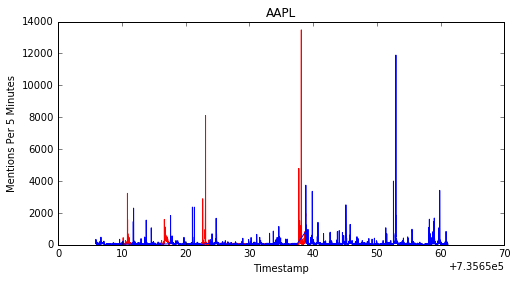
\includegraphics[scale=0.4]{img/aapl.png}
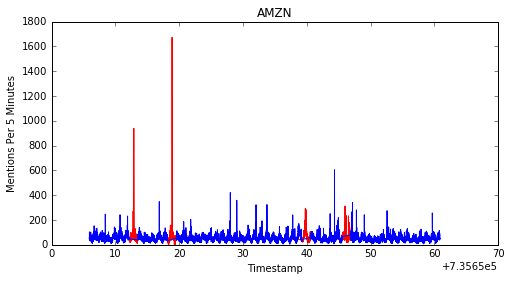
\includegraphics[scale=0.4]{img/amzn.png}
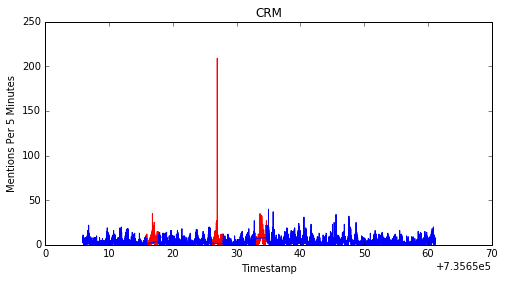
\includegraphics[scale=0.4]{img/crm.png}
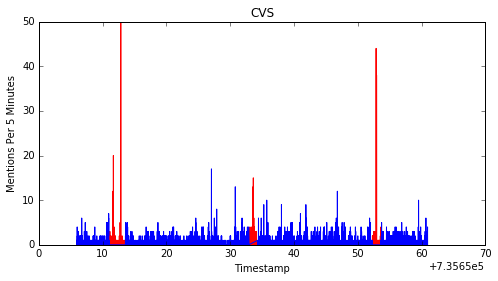
\includegraphics[scale=0.4]{img/cvs.png}
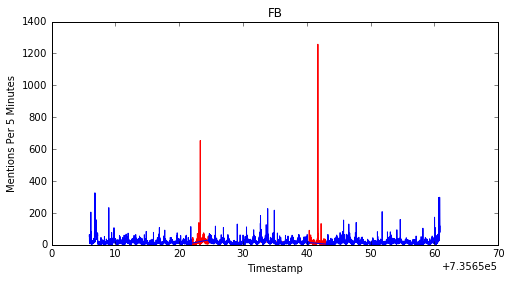
\includegraphics[scale=0.4]{img/fb.png}
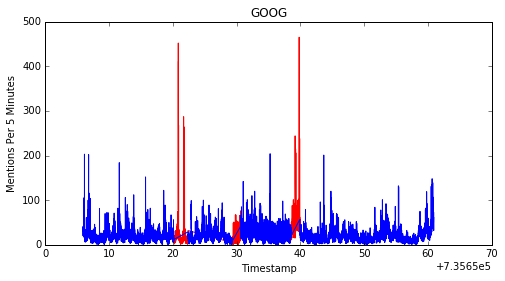
\includegraphics[scale=0.4]{img/goog.png}
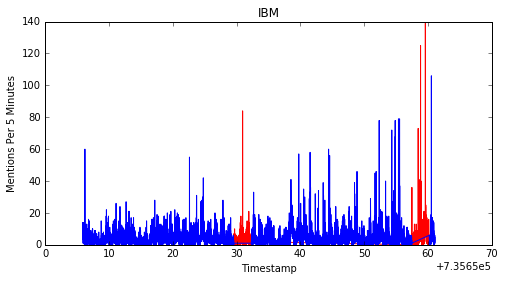
\includegraphics[scale=0.4]{img/ibm.png}
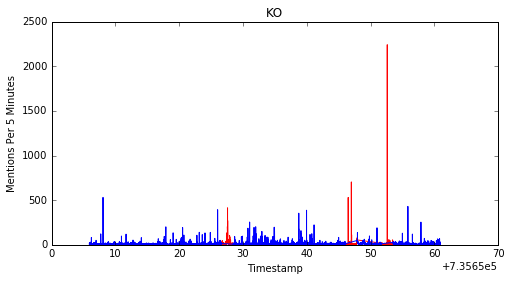
\includegraphics[scale=0.4]{img/ko.png}
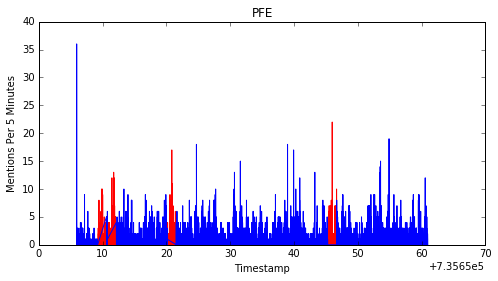
\includegraphics[scale=0.4]{img/pfe.png}
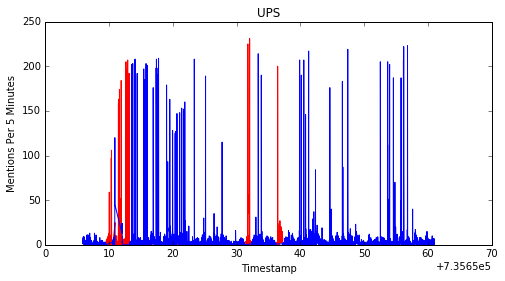
\includegraphics[scale=0.4]{img/ups.png}
\end{center}    

Note that anomalies generally correspond to a sudden peak in Twitter mentions.  However, the relationship is not always clear cut, given that there are many non-anomalous peaks and it is not always easy to tell whether or not a given rise in activity is unusual or expected.  Here are some statistics giving the mean number of mentions for anomalous and non-anomalous time frames:
\begin{center}
\begin{tabular}{ l | c c}		
  Company & Mean Mentions (Anomalous) & Mean Mentions (Non-Anomalous) \\
   \hline
GOOG & 29.1208100559 & 19.9031922276 \\
PFE & 1.30604534005 & 0.817659425368 \\
IBM & 5.52641509434 & 4.26393064392 \\
AAPL & 214.986775819 & 71.1928182199 \\
KO & 16.7971014493 & 10.7964806506 \\
CVS & 0.617955439056 & 0.332100230334 \\
FB & 18.1466498104 & 17.7740509438 \\
AMZN & 63.4063291139 & 52.1778120834 \\
UPS & 10.5621451104 & 4.88964358238 \\
CRM & 6.16886377903 & 3.03543224544 \\
\end{tabular}    
\end{center}  
\end{document}